\documentclass[12pt,a4paper]{article}
\usepackage[dutch]{babel}
\usepackage[utf8]{inputenc}
\usepackage[margin=0.5in]{geometry}
\usepackage{amsmath}
\usepackage{amsfonts}
\usepackage{amssymb}
\usepackage{graphicx}
\usepackage{listings}
\usepackage{float}
\usepackage{hyperref}



\begin{document}
\graphicspath{{images/}}
\DeclareGraphicsExtensions{.pdf,.png,.jpg}
\lstset{language=bash}
\author{Frank Willemsen}
\title{Een programma installeren met Synaptic}
\date{\today}
\maketitle
\abstract{Een beknopte inleiding tot het gebruik van Synaptic op Debian}
\section{Een programma installeren met Synaptic}


Je opent Synaptic. Dit programma vind je waarschijnlijk onder Overige. Zo niet, dan kun je altijd \emph{Opdracht uitvoeren\ldots} kiezen uit het startmenu en dan ''Synaptic'' invoeren. 

\begin{figure} [H]
\centering
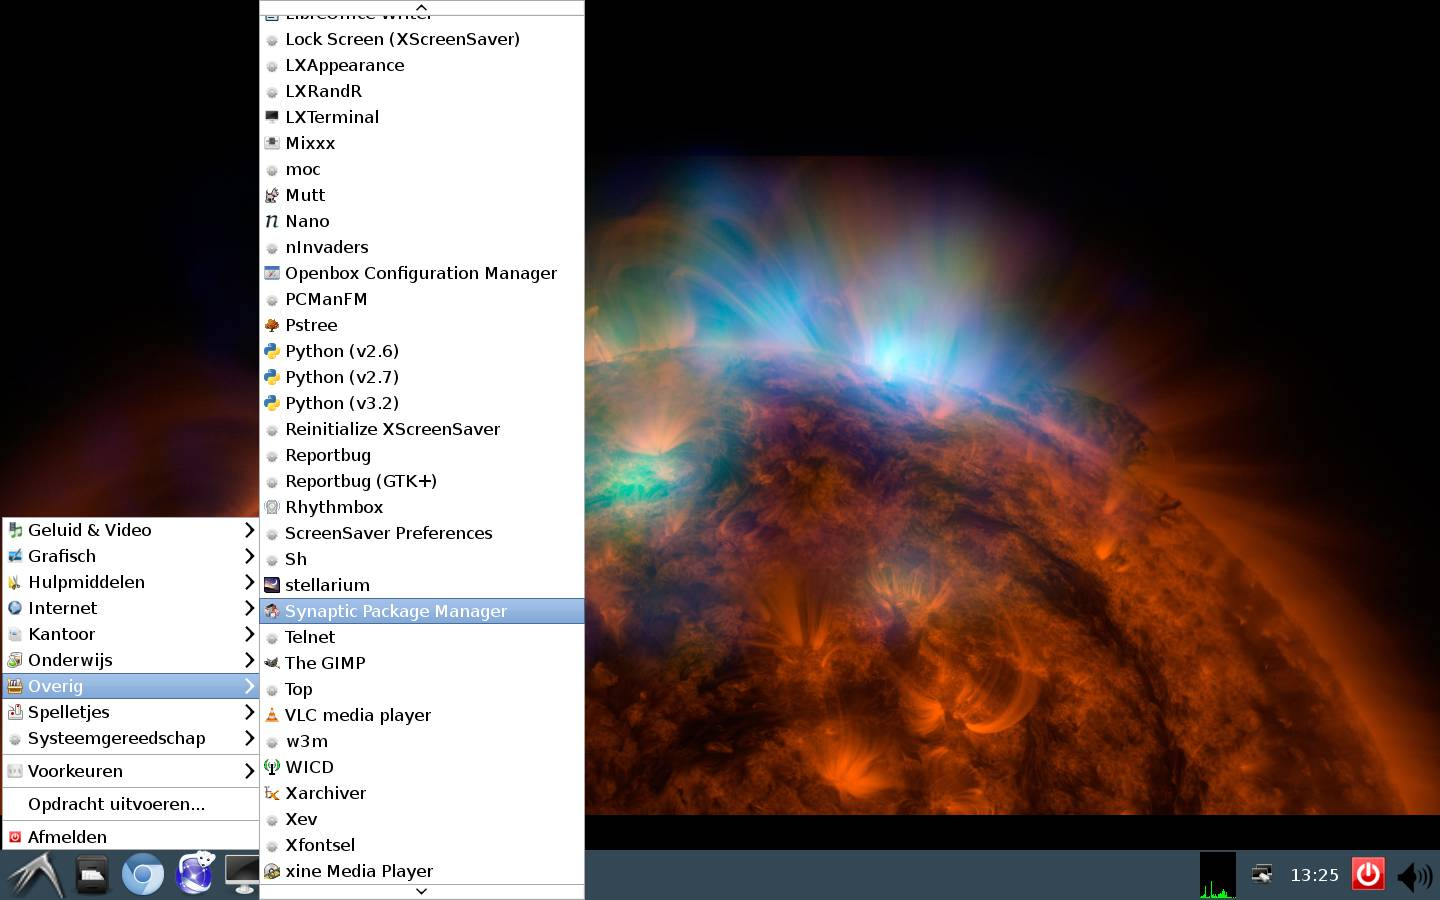
\includegraphics[width=0.6\textwidth]{plaatje01}
\caption{open Synaptic}
\label{plaatje01}
\end{figure}

Synaptic vraagt gelijk bij openen naar je wachtwoord. Het heeft dit nodig om software te kunnen installeren of te verwijderen.

\begin{figure} [H]
\centering
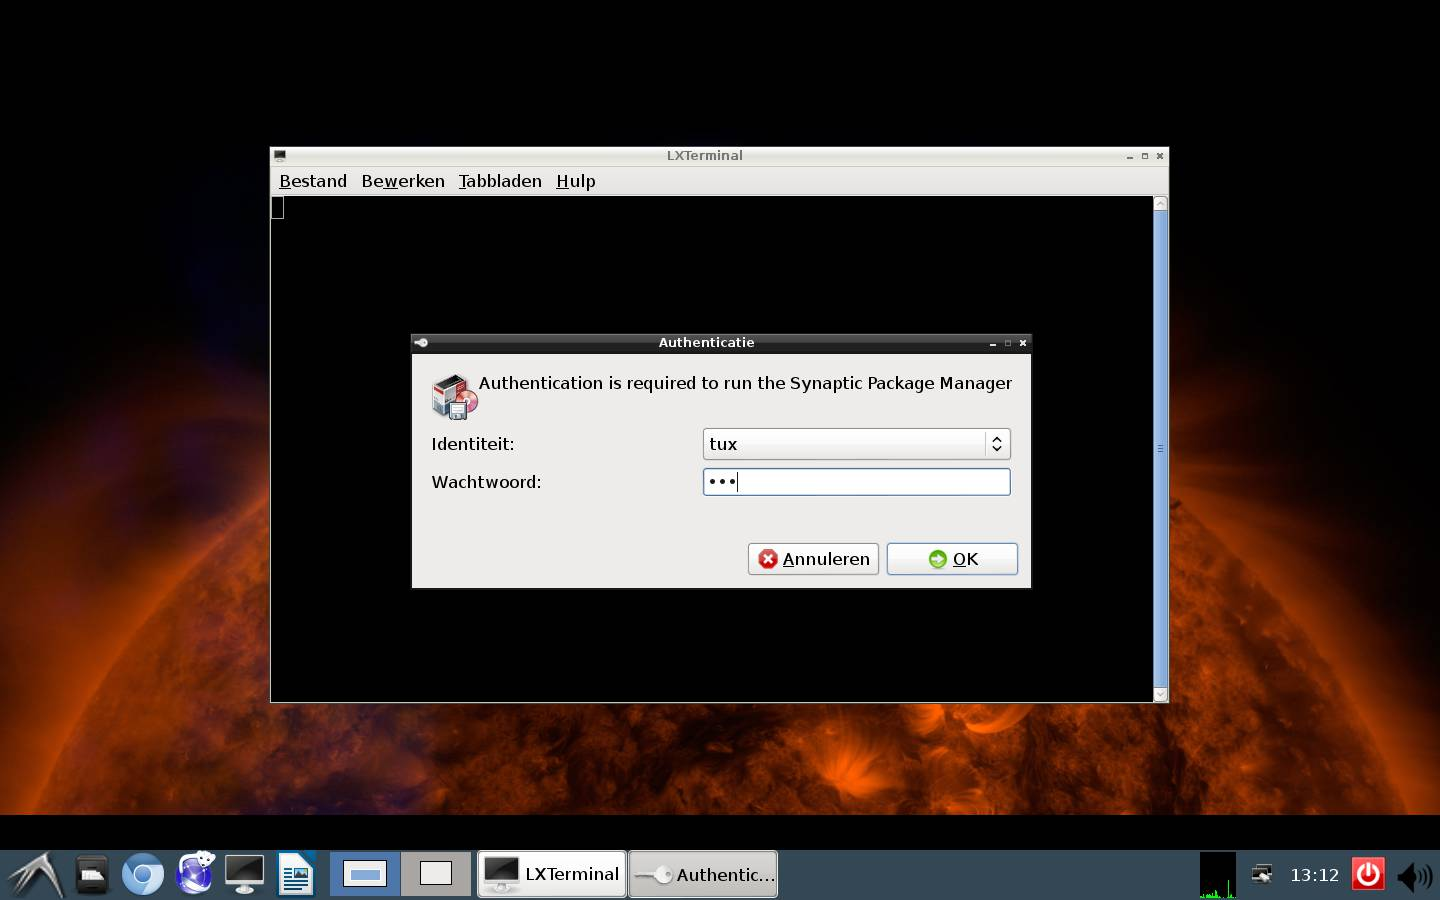
\includegraphics[width=0.6\textwidth]{plaatje02}
\caption{Wachtwoordinvoer}
\label{plaatje02}
\end{figure}

\clearpage

Nu je er toch bent, is het een goed idee om te herladen. Daarna weet je zeker dat je van alle programma's de nieuwste beschikbare versie kunt krijgen.

\begin{figure} [H]
\centering
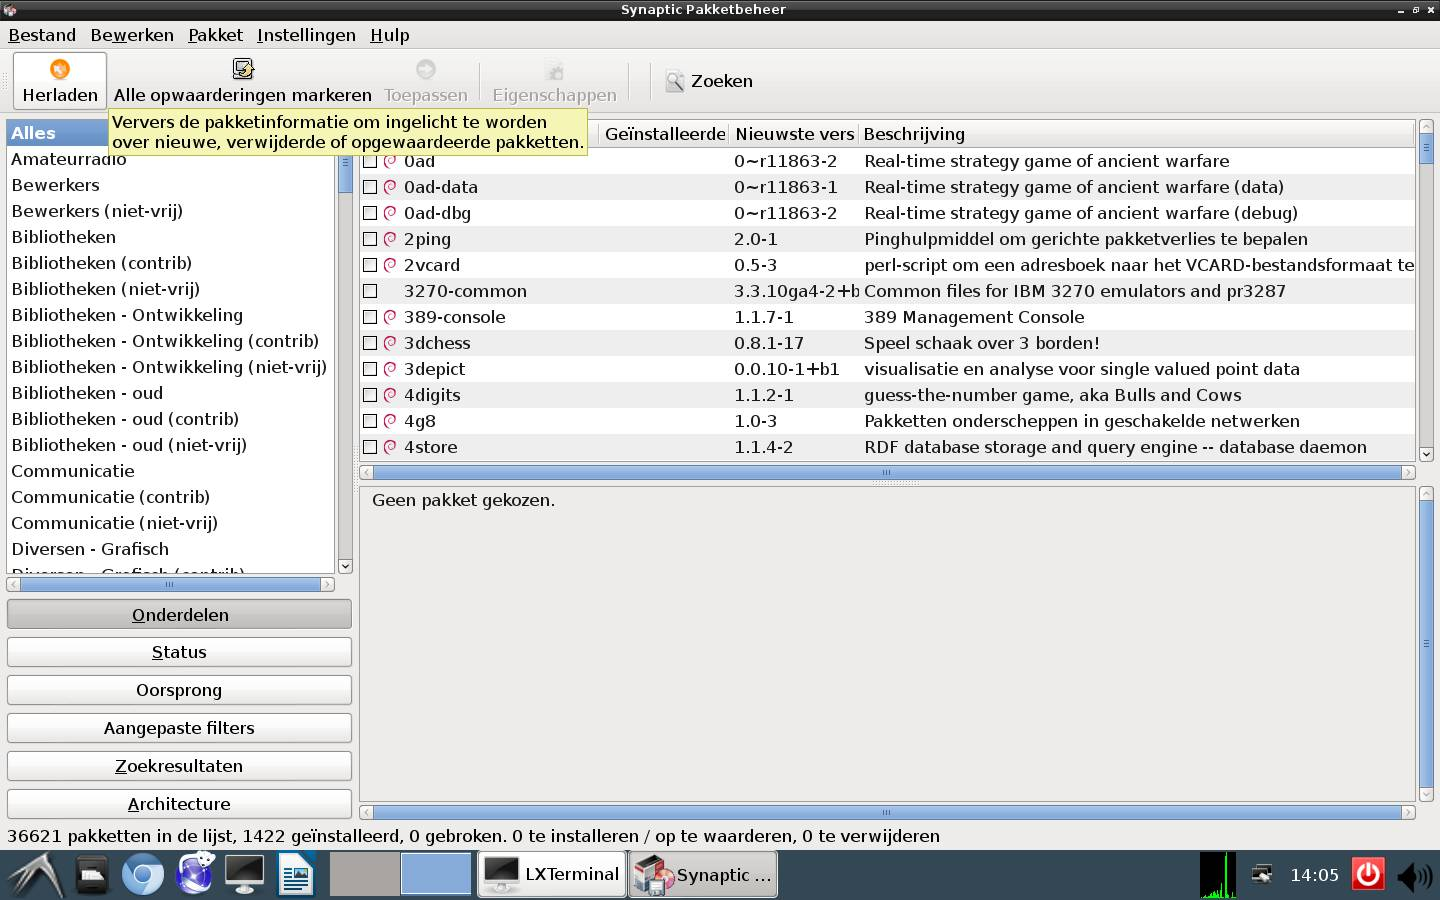
\includegraphics[width=0.45\textwidth]{plaatje04}
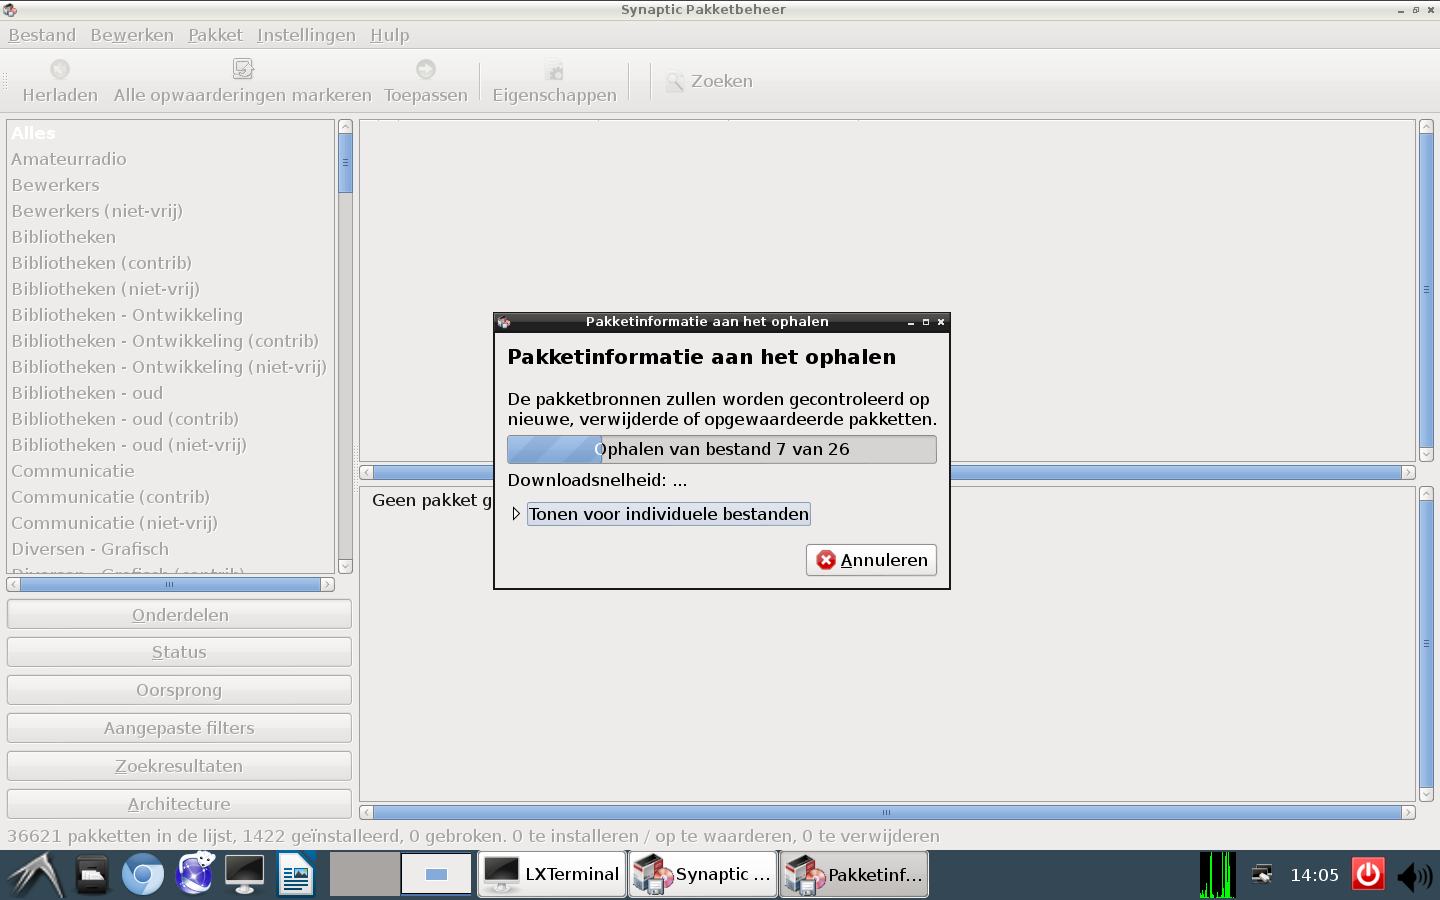
\includegraphics[width=0.45\textwidth]{plaatje05}
\caption{Pakketinformatie herladen}
\label{plaatje04}
\end{figure}

Als je weet welk programma je wilt installeren, hoef je niet moeilijk te doen en het in een menu op te zoeken. Je doet Zoeken en voert de naam in.

\begin{figure} [H]
\centering
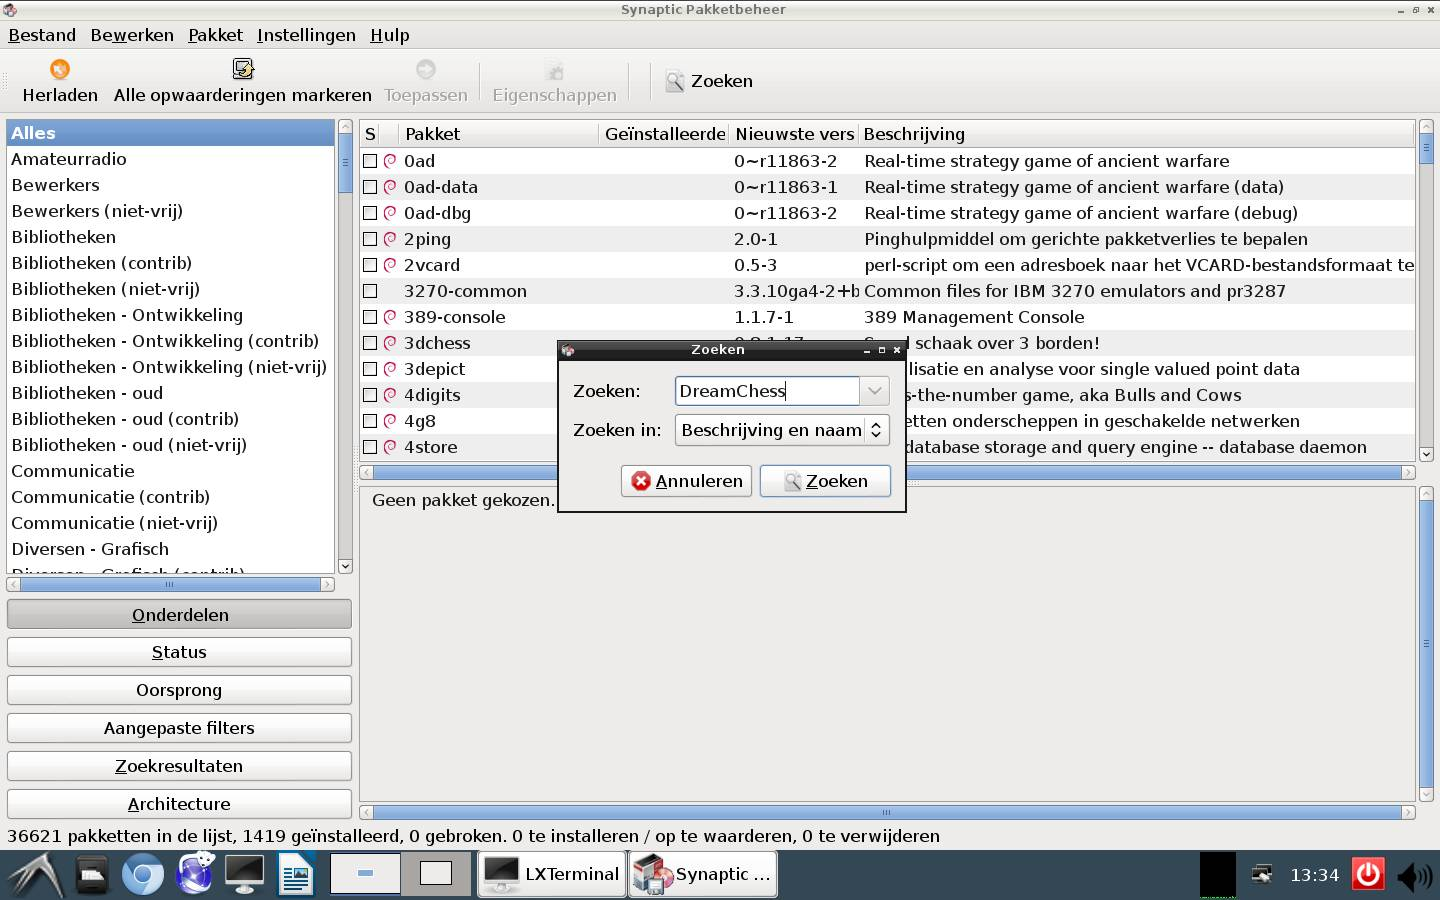
\includegraphics[width=0.6\textwidth]{plaatje06}
\caption{Zoeken naar een programma}
\label{plaatje06}
\end{figure}

In dit voorbeeld installeren we het schaakspelletje DreamChess. Dat vink je aan.	

\begin{figure} [H]
\centering
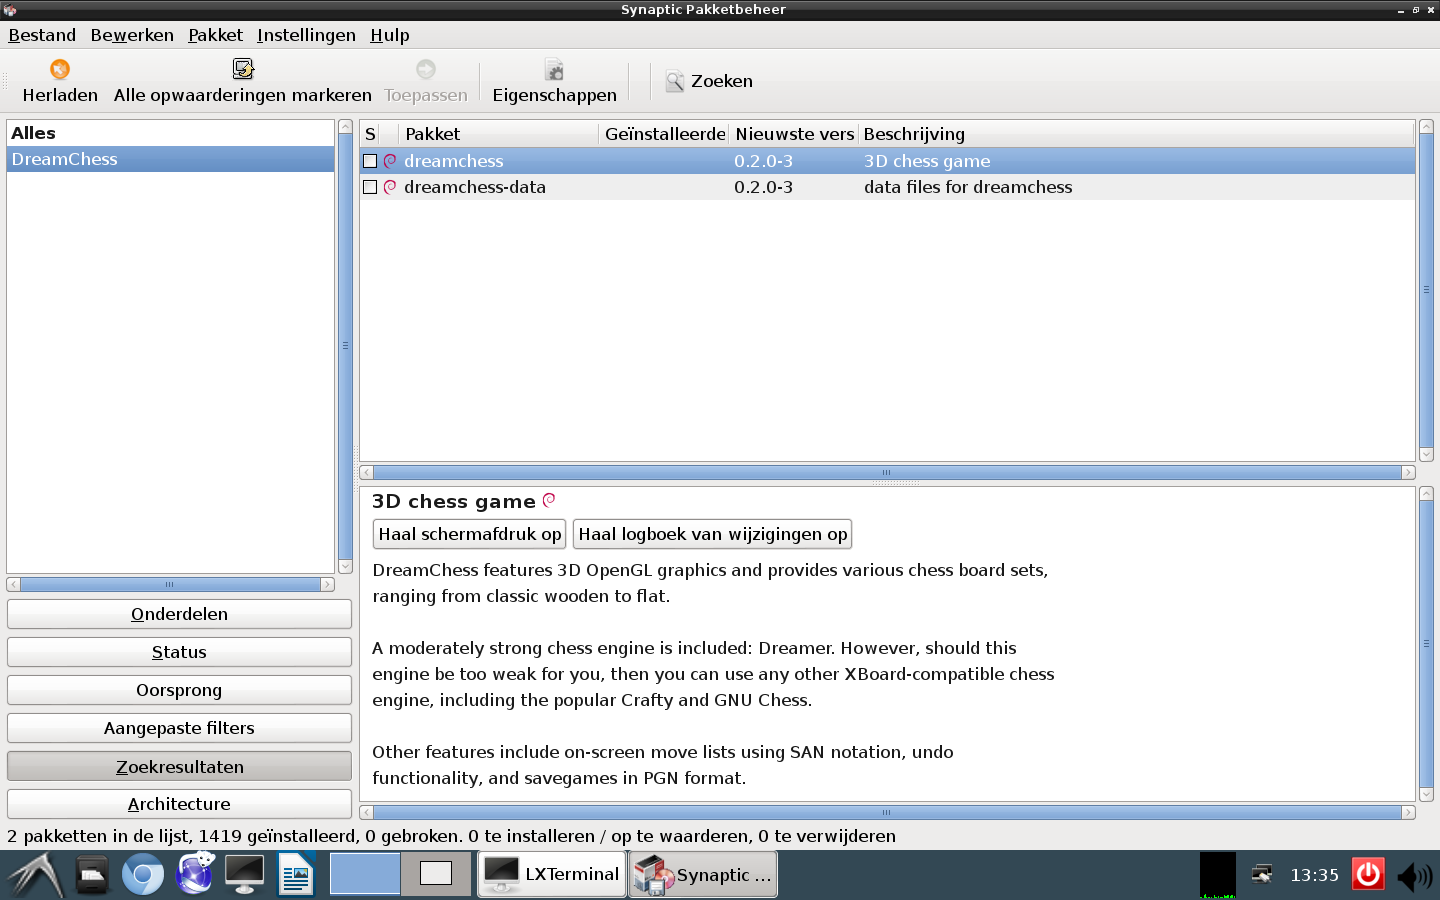
\includegraphics[width=0.6\textwidth]{plaatje07}
\caption{Selectie}
\label{plaatje07}
\end{figure}

\clearpage

DreamChess vraagt je om nog een paar andere stukjes software aan te vinken. Het functioneert niet naar behoren zonder. Dus klik je Markeren.

\begin{figure} [H]
\centering
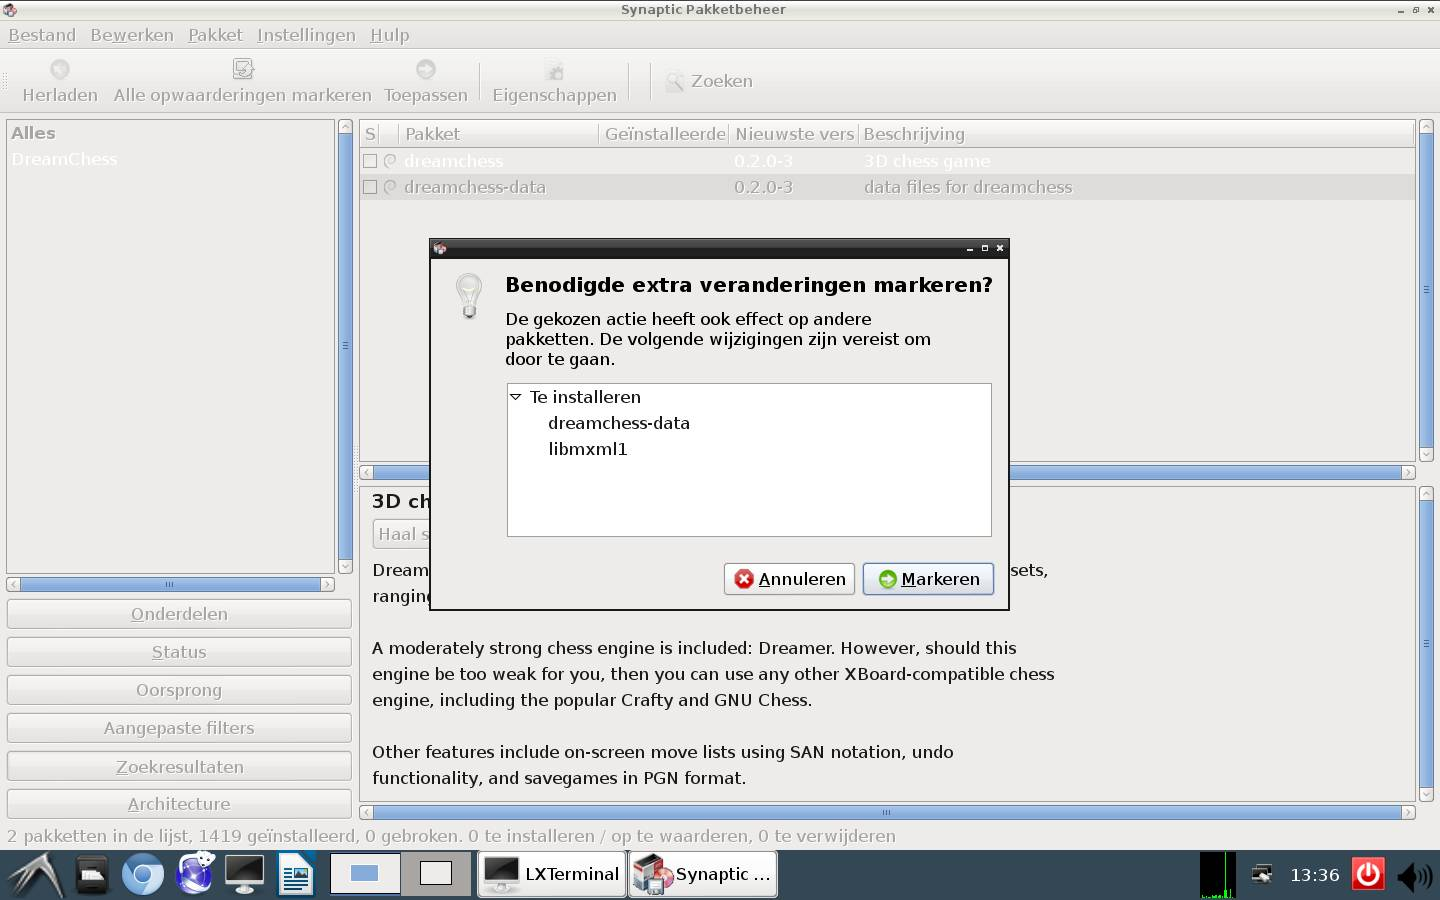
\includegraphics[width=0.6\textwidth]{plaatje08}
\caption{Benodigde extra software}
\label{plaatje08}
\end{figure}

Nu klik je Toepassen. Er wordt nog eens gevraagd of je zeker weet dat je dit wilt doen. Dus klik je opnieuw op Toepassen. 

\begin{figure} [H]
\centering
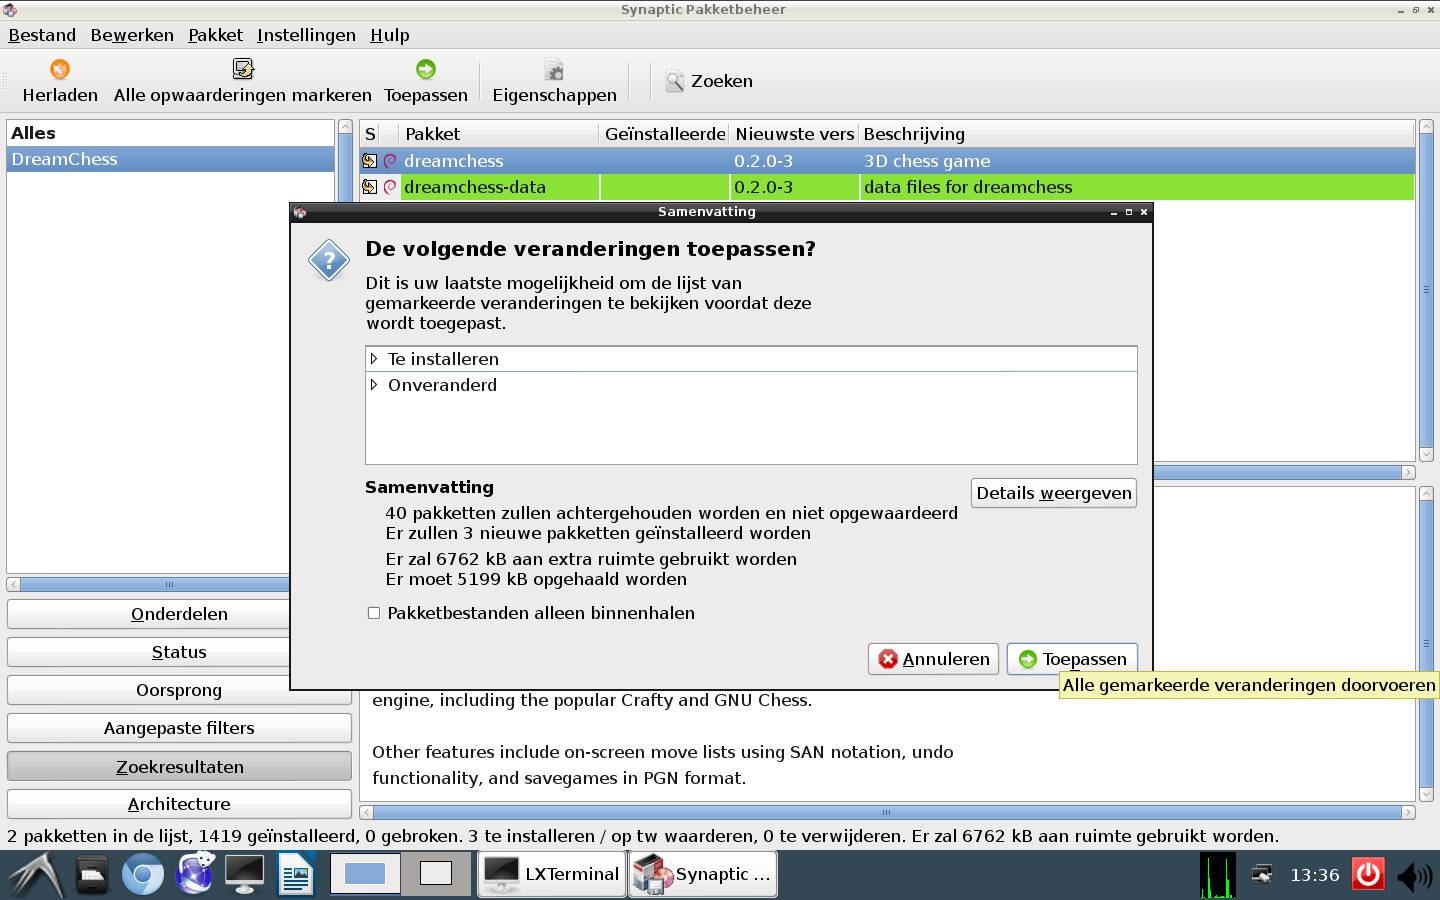
\includegraphics[width=0.6\textwidth]{plaatje10}
\caption{Kies Toepassen om je keus te bevestigen}
\label{plaatje10}
\end{figure}

Synaptic gaat nu softwarepakketten ophalen. Daarna gaat het deze installeren.

\begin{figure} [H]
\centering
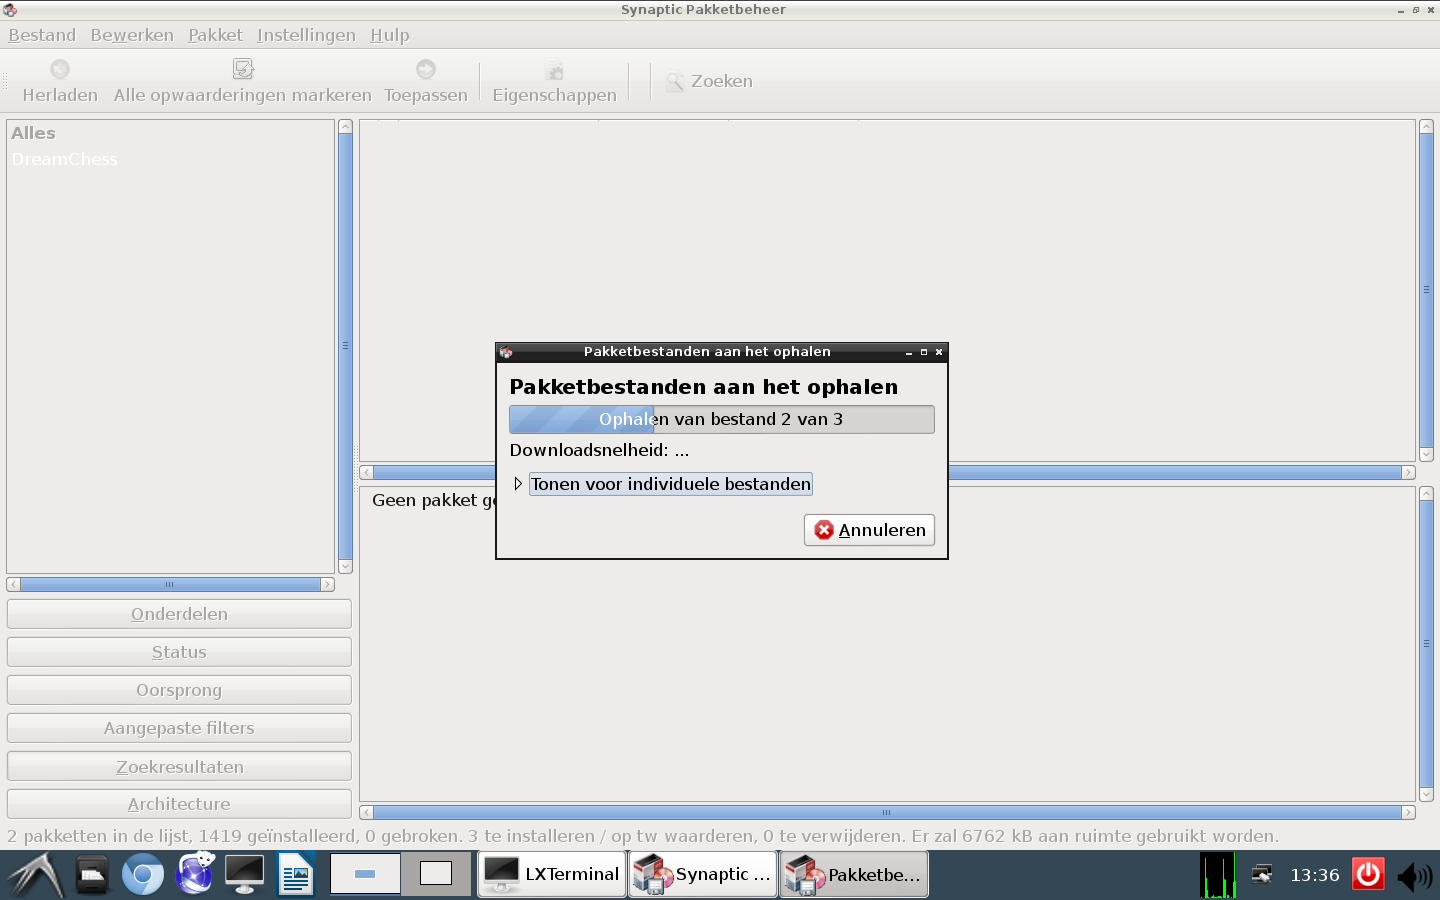
\includegraphics[width=0.45\textwidth]{plaatje11}
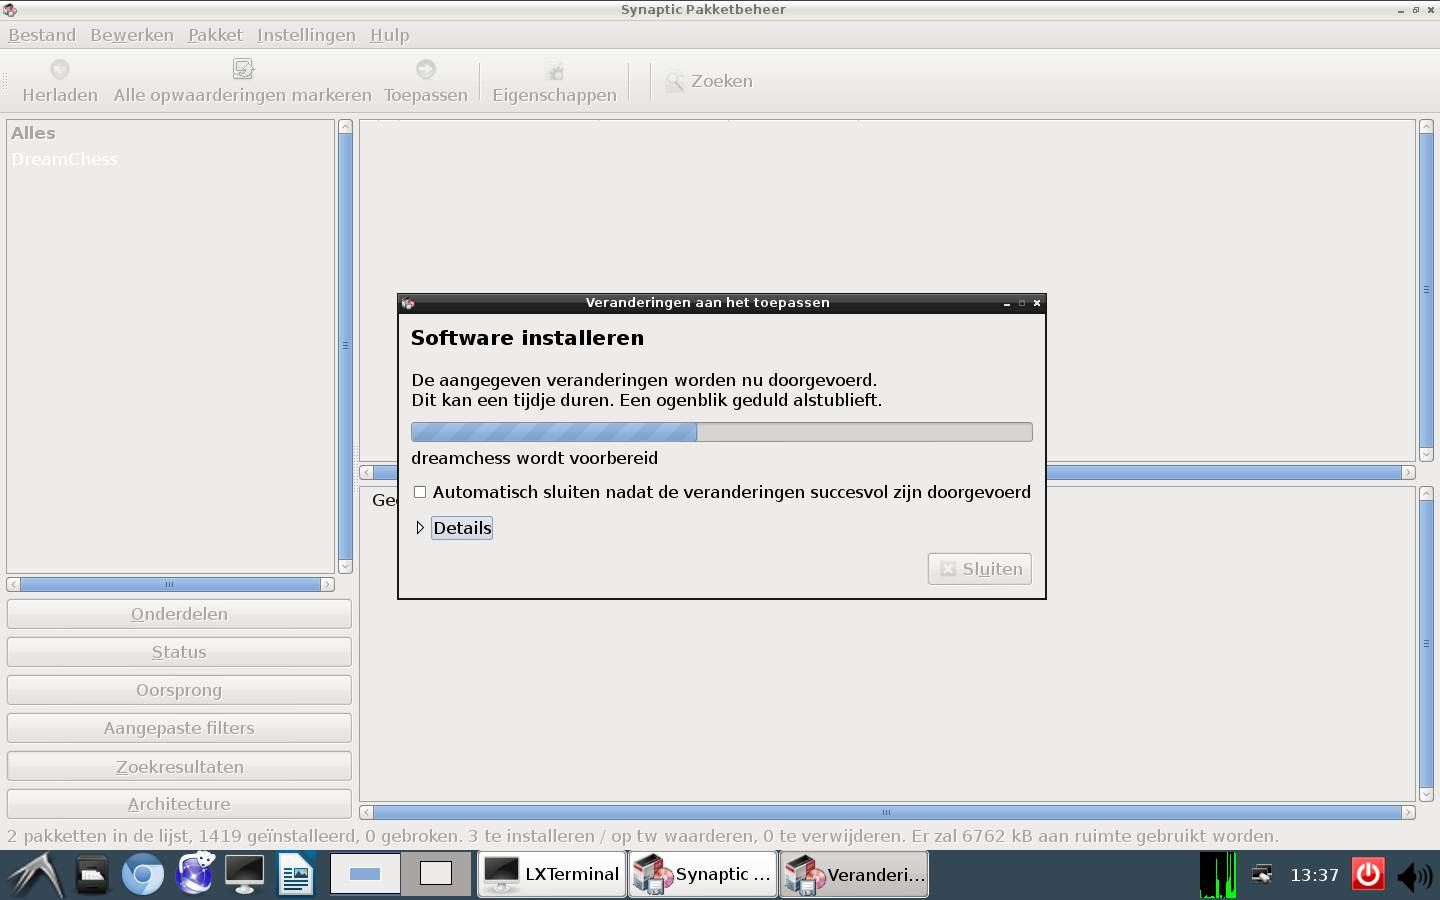
\includegraphics[width=0.45\textwidth]{plaatje12}
\caption{download en installatie}
\label{plaatje11}
\end{figure}

\clearpage

Als het geslaagd is, kun je daarna Synaptic afsluiten.

\begin{figure} [H]
\centering
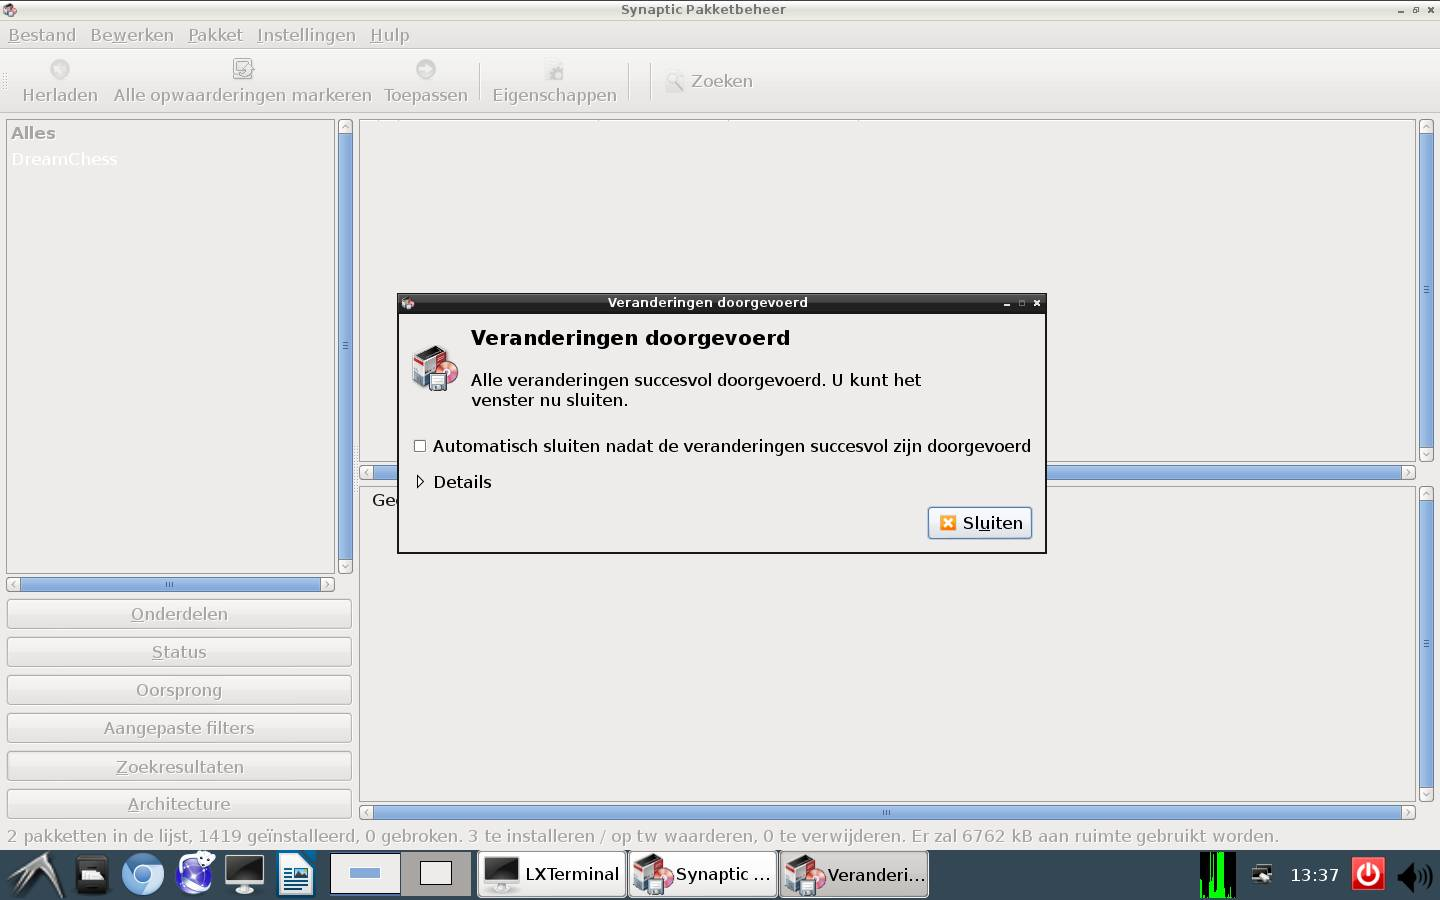
\includegraphics[width=0.6\textwidth]{plaatje13}
\caption{Klaar!}
\label{plaatje13}
\end{figure}

In Debian blijkt Dream Chess ondergebracht te zijn onder Spelletjes. We zijn klaar voor een potje schaak!

Mocht je het niet gelijk kunnen terugvinden, kies dan \emph{Opdracht uitvoeren\ldots} uit het startmenu en voer ''DreamChess'' in.

\begin{figure} [H]
\centering
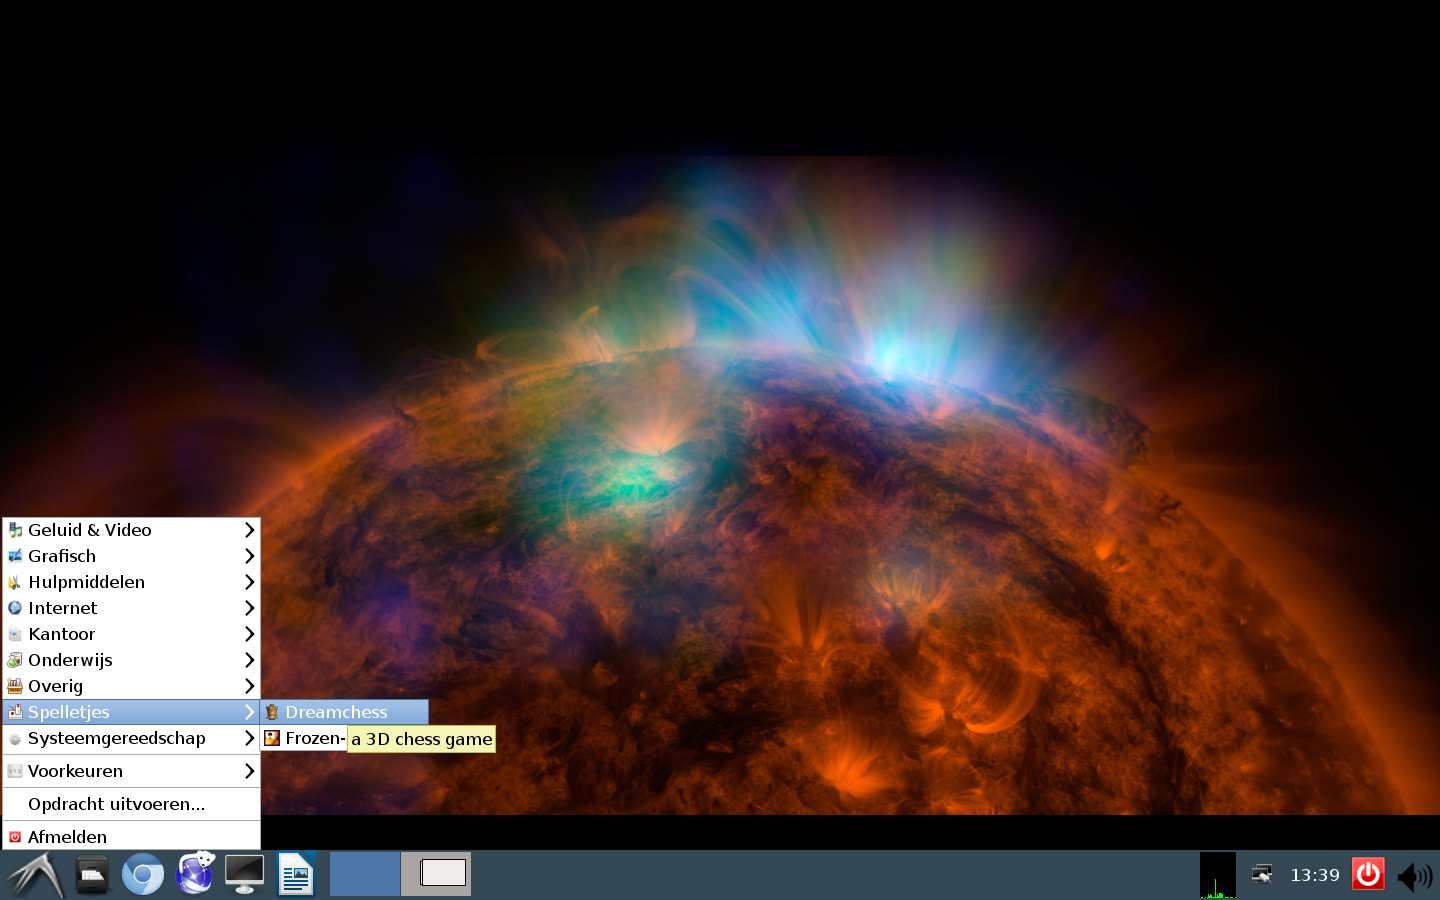
\includegraphics[width=0.45\textwidth]{plaatje14}
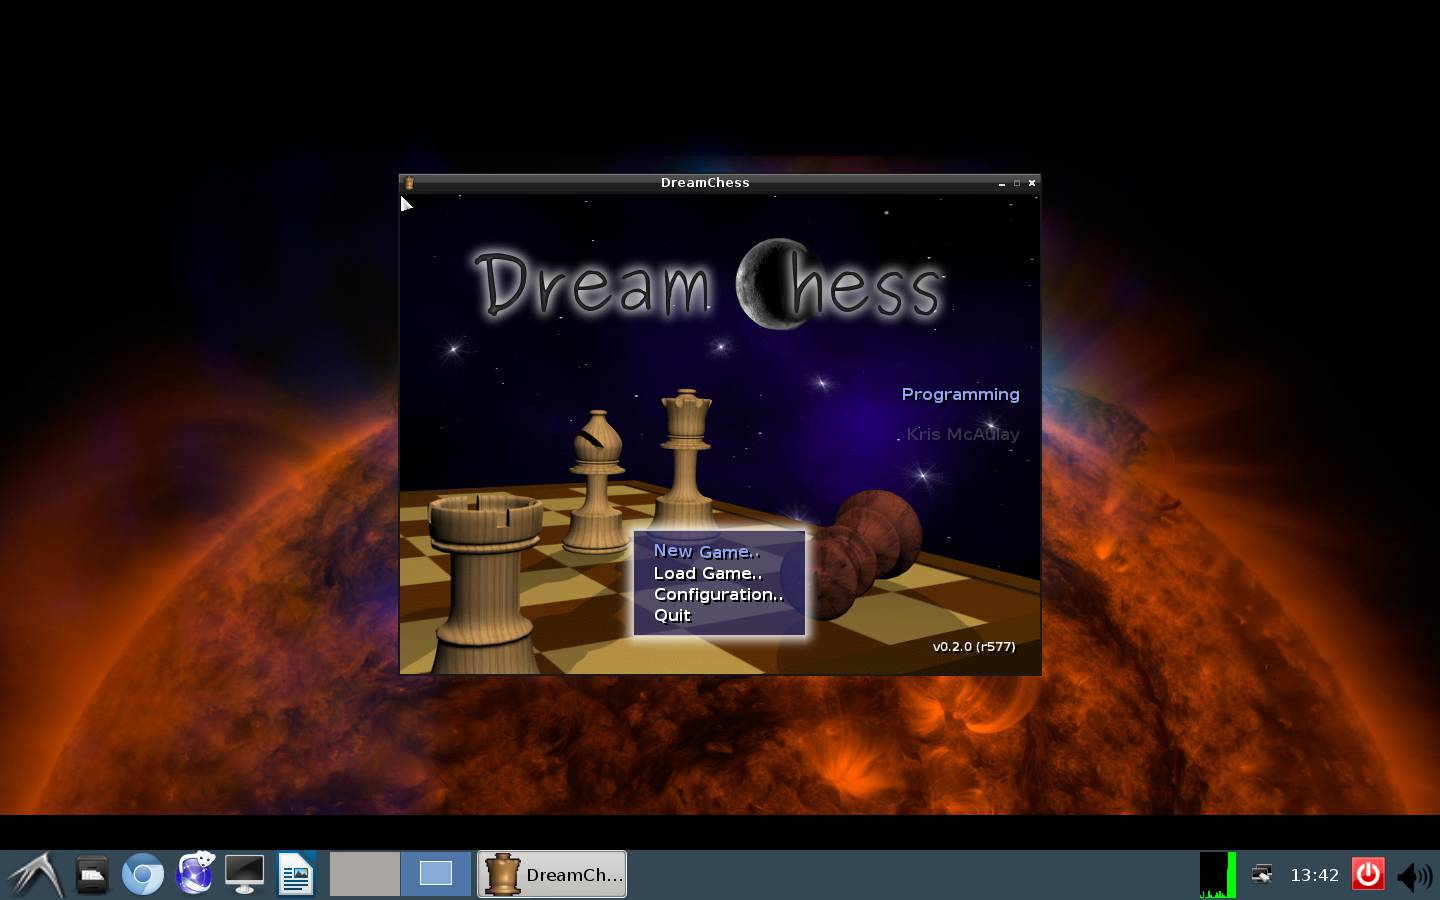
\includegraphics[width=0.45\textwidth]{plaatje15}
\caption{DreamChess is ge\"{i}nstalleerd}
\label{plaatje14}
\end{figure}

\end{document}
